% "{'chapitre':'slci_laplace','classe':('PSI'),'type':('colle','td'),'titre':'Gyropode à usage professionnel HUBLEX', 'source':'Concours CCINP - MP 2020','comp':('B2-04','C2-03'),'corrige':False}"

%\setchapterimage{fig_00}
\renewcommand{\titrechapitre}{Gyropode à usage professionnel HUBLEX}
\renewcommand{\leftmark}{\titrechapitre}
\renewcommand{\rightmark}{\titrechapitre}


\ifcolle
\chapter*{Colle \arabic{cptColle} \\ 
\titrechapitre -- \ifprof Corrigé \else Sujet \fi}
\addcontentsline{toc}{section}{Colle \arabic{cptColle} : \titrechapitre -- \ifprof Corrigé \else Sujet \fi}
\iflivret \stepcounter{cptColle} \else
\ifprof  \stepcounter{cptColle} \else \fi
\fi
\else
\chapter*{TD \arabic,td{cptTD} \\ 
\titrechapitre -- \ifprof Corrigé \else Sujet \fi}
\addcontentsline{toc}{section}{TD \arabic{cptTD} : \titrechapitre -- \ifprof Corrigé \else Sujet \fi}
\iflivret \stepcounter{cptTD} \else
\ifprof  \stepcounter{cptTD} \else \fi
\fi
\fi

\setcounter{question}{0}

\marginnote{Concours CCINP -- MP 2020.}
\marginnote{\UPSTIcompetence[2]{B2-04}
\UPSTIcompetence[2]{C2-03}}
\begin{marginfigure}
\centering
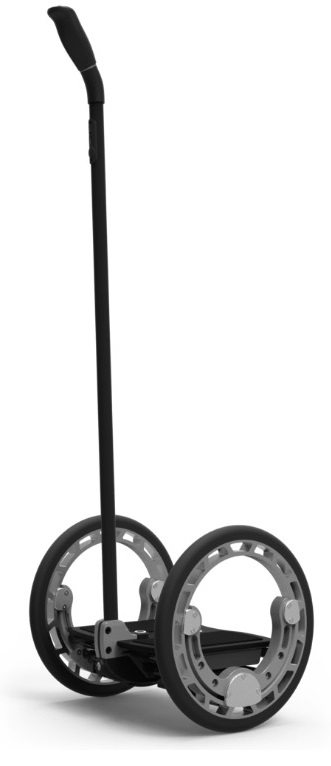
\includegraphics[width=.45\linewidth]{fig_01}
\end{marginfigure}




\subsection*{Présentation}
\ifprof
\else

Le système étudié dans ce sujet, appelé Hublex, est un gyropode professionnel destiné à faciliter le déplacement des collaborateurs au sein d’entreprises, administrations, hôpitaux... lorsque ces lieux sont de grandes tailles.
\fi

\subsection*{Étude de l’asservissement en intensité des moteurs}
\ifprof
\else

\begin{obj}
Modéliser la chaîne d’asservissement en intensité du moteur afin de déterminer les paramètres du correcteur permettant de respecter l’exigence «~1.7.1.1~» et ses sous-exigences.
\end{obj}

\begin{figure}[H]
\centering
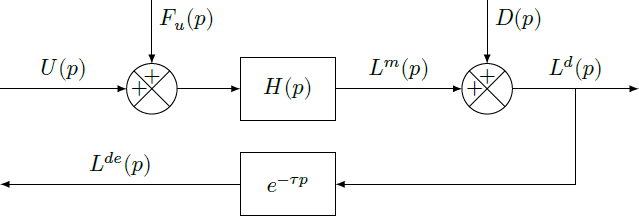
\includegraphics[width=.8\linewidth]{fig_02}
\caption{Diagramme des exigences \label{fig_02}}
\end{figure}
\fi


\subsubsection*{Modélisation du moteur}

%Le moteur brushless associé à son électronique de commande peut se modéliser par les équations d’une machine à courant continu. Les paramètres du modèle associés ont une résistance interne $R$ (en $\Omega$), une inductance $L$ (en H) et un coefficient de couplage $K_e$ (en \si{V.s.rad^{-1}} ou en \si{N.m.A^{-1}}).
%On notera $i(t)$ l’intensité traversant l’induit (en A), $u(t)$ la tension aux bornes de l’induit (en V), $e(t)$
%la force contre-électromotrice (en V), $C_m(t)$ le couple utile délivré par l’action du stator du moteur
%sur l’arbre (en \si{N.m}) et $\omega_m(t)$ la vitesse de rotation de l’arbre moteur (en \si{rad.s^{-1}}). Dans le domaine
%de Laplace, ces grandeurs seront notées respectivement $I(p)$, $U(p)$, $E(p)$, $C_m(p)$ et $\Omega_m(p)$, avec $p$ la
%variable dans le domaine de Laplace. On se place dans les conditions d’Heaviside.
\ifprof
\else

Le moteur brushless associé à son électronique de commande peut se modéliser par les équations d’une machine à courant continu. 


On notera $\indice{J}{eq}$ l’inertie équivalente des masses mobiles mises en jeu ramenée sur l’arbre moteur. On
modélisera les différents frottements par un frottement visqueux générant un couple résistant, rapporté
à l’arbre moteur, proportionnel à la vitesse de rotation de l’arbre moteur et de coefficient $f$ ($f > 0$).
On rappelle les équations caractéristiques associées :
\begin{itemize}
\item $u(t) = e(t)+Ri(t)+L\dfrac{\dd i(t)}{\dd t}$;
\item $e(t)=K_e\omega_m(t)$;
\item $C_m(t)=K_e i(t)$;
\item $\indice{J}{eq} \dfrac{\dd \omega_m(t)}{\dd t} = C_m(t)-f\omega_m(t)$.
\end{itemize}
\fi


\question{Donner, dans le domaine de Laplace, les 4 équations caractéristiques associées au modèle de
machines à courant continu.}
\ifprof
\begin{corrige}
\begin{itemize}
\item $U(p) = E(p)+RI(p)+Lp I(p)$;
\item $E(p)=K_e\Omega_m(p)$;
\item $C_m(p)=K_e I(p)$;
\item $\indice{J}{eq} p\Omega_m(p) = C_m(p)-f\Omega_m(p)$.
\end{itemize}
\end{corrige}
\else
\fi

\ifprof
\else
\begin{marginfigure}
\centering
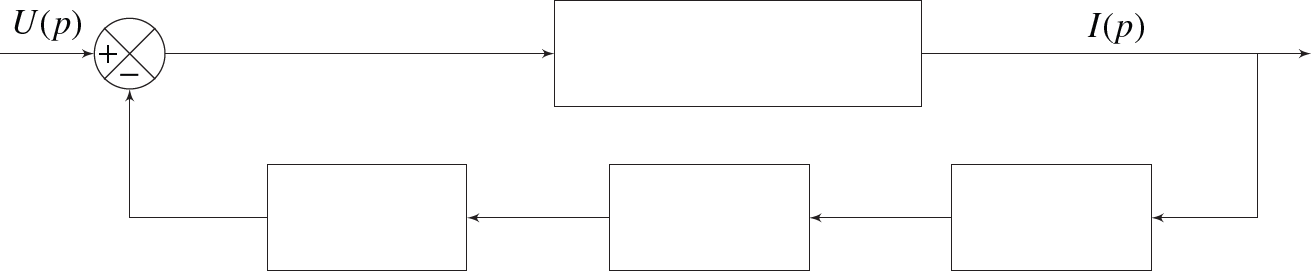
\includegraphics[width=\linewidth]{fig_dr3}
\caption{Schéma-blocs \label{fig_dr3}}
\end{marginfigure}
\fi


\question{Compléter alors le schéma-blocs du moteur dans \autoref{fig_dr3}. On précisera la grandeur associée à
chaque lien.}
\ifprof
\begin{corrige}
\begin{center}
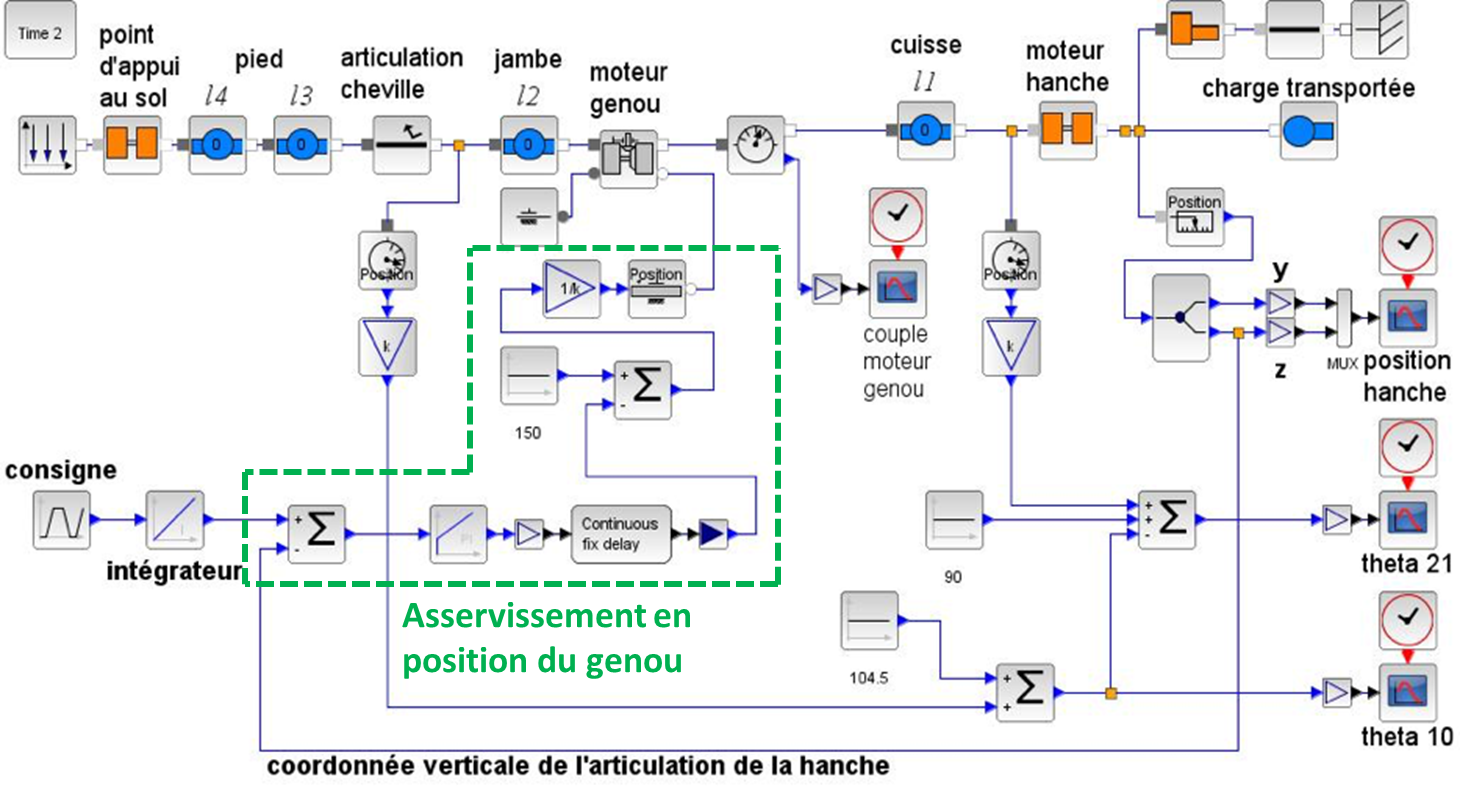
\includegraphics[width=10cm]{cor_01}
\end{center}
\end{corrige}
\else
\fi


\question{Donner l’expression de la fonction de transfert $H_m(p)=\dfrac{I(p)}{U(p)}$. Mettre cette fonction de transfert sous la forme $H_m(p)=K_m\dfrac{1+\tau_m p}{1+\dfrac{2z_m}{\omega_{0m}}p+\dfrac{1}{\omega_{0m}^2}p^2}$.}
\ifprof
\begin{corrige}
En utilisant la formule de Black, on a 
$H_m(p)=\dfrac{I(p)}{U(p)} = \dfrac{\dfrac{1}{R+Lp}}{1+K_e^2 \dfrac{1}{R+Lp} \dfrac{1}{f+Jp}}$
$ = \dfrac{1}{\left(R+Lp\right)+K_e^2 \dfrac{1}{f+Jp}}$
$ = \dfrac{f+Jp}{\left(R+Lp\right)\left(f+Jp\right)+K_e^2 }$

$ = \dfrac{f+Jp}{Rf+\left(Lf + RJ\right)p+LJp^2 +K_e^2 }$
$ = \dfrac{f}{Rf+K_e^2} \dfrac{1+\dfrac{J}{f}p}{\left(Lf + RJ\right)\dfrac{p}{Rf+K_e^2}+\dfrac{LJp^2}{Rf+K_e^2}+1 }$.

On a donc $K_m = \dfrac{f}{Rf+K_e^2}$, $\tau_m=\dfrac{J}{f}$, 
$\dfrac{1}{\omega_{0m}^2} = \dfrac{LJ}{Rf+K_e^2} \Rightarrow \omega_{0m} = \sqrt{\dfrac{Rf+K_e^2}{LJ}} $
et $ \dfrac{2z_m}{\omega_{0m}} = \dfrac{Lf + RJ}{Rf+K_e^2} \Rightarrow z_m = \dfrac{\omega_{0m}}{2}\dfrac{Lf + RJ}{Rf+K_e^2}$
$\Rightarrow z_m = \dfrac{Lf + RJ}{2\sqrt{LJ}\sqrt{Rf+K_e^2}}$.

\end{corrige}
\else
\fi


\subsection*{Asservissement du moteur en intensité}
\ifprof
\else

\begin{marginfigure}
\centering
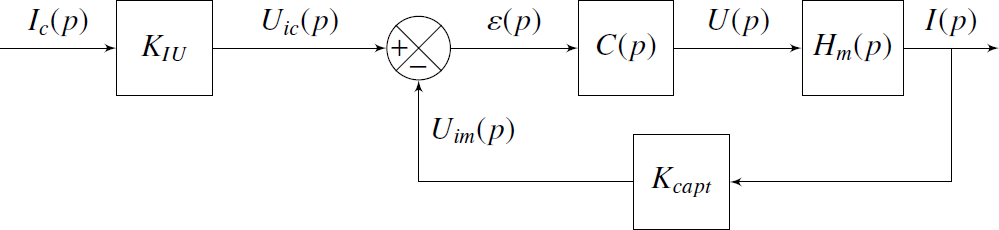
\includegraphics[width=\linewidth]{fig_13}
\caption{Schéma-blocs \label{fig_13}}
\end{marginfigure}

L’architecture retenue pour contrôler le couple moteur est un asservissement en intensité, image du
couple moteur (voir équation précédente). Le schéma-blocs est représenté \autoref{fig_13}. Un convertisseur IU
fournit au calculateur une tension $\indice{u}{ic}(t)$ image de l’intensité de consigne $i_c(t)$, proportionnelle à cette
dernière de coefficient $\indice{K}{iu}$. De même, l’intensité réelle $i(t)$, mesurée par un capteur d’intensité de
coefficient $\indice{K}{capt}$, a pour image $\indice{u}{im}(t)$. L’écart, noté $\varepsilon(t) = \indice{u}{ic}(t) - \indice{u}{im}(t)$, est traité par le correcteur de fonction de transfert $C(p)$, qui impose la tension $u(t)$ aux bornes du moteur.
%On note $I_c(p)$, $\indice{U}{ic}(p)$, $\indice{U}{im}(p)$, $\varepsilon(p)$ les transformées de Laplace respectives de $i_c(t)$, $\indice{u}{ic}(t)$, $\indice{u}{im}(t)$ et $\varepsilon(t)$.

On donne la fonction de transfert du moteur : $H_m(p)=K_m\dfrac{1+\tau_m p}{1+\dfrac{2z_m}{\omega_{0m}}p+\dfrac{1}{\omega_{0m}^2}p^2}$.

\fi

\question{Préciser, en justifiant, quelle valeur donner à $\indice{K}{iu}$, caractéristique du convertisseur IU.}
\ifprof
\begin{corrige}

Pour avoir $\varepsilon = 0$ lorsque $I_c(p)=I(p)$, il faut nécessairement $\indice{K}{capt}=\indice{K}{IU}$.
\end{corrige}
\else
\fi

\ifprof
\else

On prend, dans un premier temps, un correcteur purement proportionnel: $C(p)=K_p$.

On en déduit la fonction de transfert $H_I(p)=\dfrac{I(p)}{I_c(p)}$ :

$H_I(p)=\dfrac{K'}{1+K'}\dfrac{1+\tau_m p}{1+  
\dfrac{\dfrac{2z_m}{\omega_{0m}}+ K'\tau_m}{1+K'}p 
+ \dfrac{1}{\omega_{0m}^2(1+K')} p^2}$, avec $K'=\indice{K}{iu}K_pK_m$.

\fi

\question{Calculer l’expression littérale de l’erreur en régime permanent notée $\mu_s$, pour une entrée indicielle (i.e. $I_c(p)$ est un échelon unitaire), en fonction de $\indice{K}{iu}$, $\indice{K}{p}$ et $K_m$.}
\ifprof
\begin{corrige}
$\indice{K}{capt}=\indice{K}{IU}$, il est donc possible de positionner $\indice{K}{capt}$ en amont de la chaîne directe, de supprimer $\indice{K}{IU}$ et de se ramener à un schéma-blocs à retour unitaire. 

On a alors $\text{FTBO}(p)=\indice{K}{Capt}C(p)H_m(p)$ et 
$\varepsilon(p)=\dfrac{I_c(p)}{1+\text{FTBO}(p)}$.

On a alors $\varepsilon_s = \lim\limits_{p \to 0 } p\times\dfrac{1}{p}\dfrac{1}{1+\text{FTBO}(p)}$  
$= \lim\limits_{p \to 0 } \dfrac{1}{1+\text{FTBO}(p)} = \dfrac{1}{1+K_m K_P \indice{K}{Capt}} $.
\end{corrige}
\else
\fi

%\ifprof
%\else
%
%La \autoref{fig_14} présente les diagrammes de Bode en boucle ouverte de l’asservissement étudié, en prenant $K_p=10$.
%
%\begin{figure}[H]
%\centering
%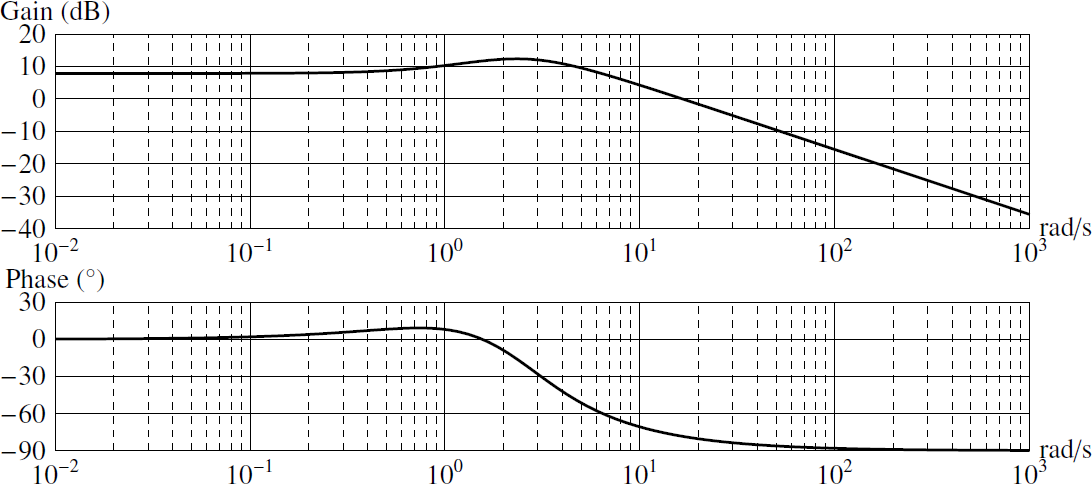
\includegraphics[width=.8\linewidth]{fig_14}
%\caption{Diagrammes de Bode en boucle ouverte pour $K_p = 10$\label{fig_14}}
%\end{figure}

%\fi

%Q30.
\question{Conclure, lorsque cela est possible, quant au respect des sous exigences de l’exigence «~1.7.1.1.1~» avec ce type de correcteur.}
\ifprof
\begin{corrige}
Avec ce correcteur, l'exigence de précision nulle ne pourra pas être satisfaite.
\end{corrige}
\else
\fi

\ifprof
\else

Dans un deuxième temps, il est décidé d’utiliser un correcteur de type proportionnel intégral. Sa fonction de transfert est notée : $C(p)=K_p+\dfrac{K_i}{p}$.
\fi

%%Q31.
%\question{Préciser l’influence de cecorrecteur sur les performances du système. Justifier le choix de ce type de correcteur dans le cas étudié.}
%
%On souhaite régler le correcteur afin de respecter les performances de précision et de stabilité.
%
%%Q32.
\question{Tracer  les diagrammes de Bode asymptotique du correcteur ainsi que l’allure des courbes réelles pour $K_p=10$ et $K_i=1000$. On précisera les valeurs numériques associées aux valeurs caractéristiques.}

\ifprof
\begin{corrige}

$C(p)=K_p+\dfrac{K_i}{p}=\dfrac{K_p p + K_i}{p} = K_i \dfrac{\dfrac{K_p}{K_i} p +1 }{p}$
$=\dfrac{1000}{p}\left(\dfrac{1}{100}p+1\right)$. 

On peut donc dresser le tableau de variation asymptotique.

\begin{figure}[H]
\centering
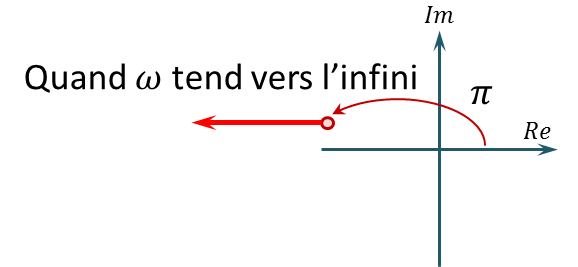
\includegraphics[width=.7\linewidth]{cor_02}
%\caption{Schéma-blocs \label{cor_02}}
\end{figure}

L'asymptote du gain décibel de << $H_1(p)$ >> coupe l'axe des abscisses en 1000.

\begin{figure}[H]
\centering
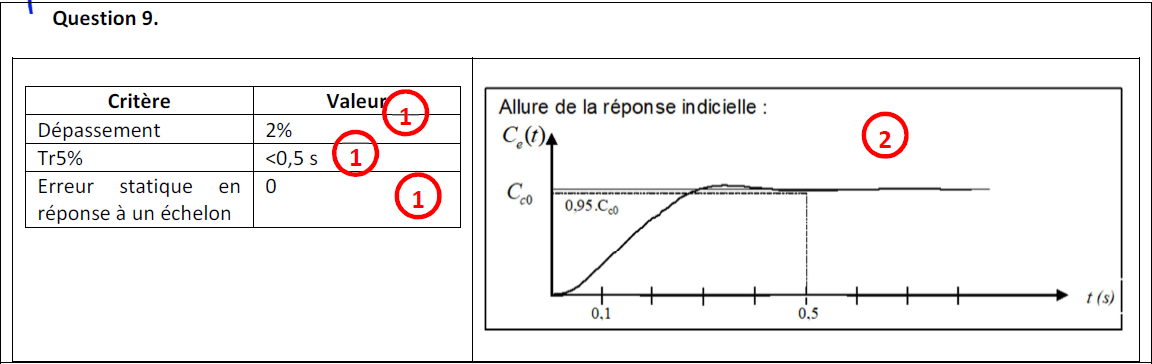
\includegraphics[width=.7\linewidth]{cor_03}
%\caption{Schéma-blocs \label{cor_02}}
\end{figure}


\end{corrige}
\else
\fi


% On se propose de régler le correcteur grâce à la méthode suivante, en deux étapes :}
%\textit{\begin{enumerate}
%\item réglage de $K_p$ seul (c’est-à-dire en considérant $K_i=0$ tout d’abord), de façon à respecter les exigences de stabilité et de bande passante;
%\item  réglage de $K_i$ de façon à éloigner la pulsation de cassure du correcteur à une décade vers la gauche de la pulsation de coupure à \SI{0}{dB}, de manière à ce que $\SI{0}{dB}$ ne soit quasiment pas modifiée.
%\end{enumerate}}
%
%%Q33.
%\question{En suivant cette méthode, déterminer en justifiant la valeur numérique de $K_p$.}
%
%%Q34.
%\question{Déterminer alors la valeur numérique de $K_i$.}

\ifprof
\else
 Une fois le correcteur réglé, on obtient les diagrammes de Bode en boucle ouverte (\autoref{fig_15}) et les réponses temporelles (\autoref{fig_16}), pour un échelon d’intensité $i_c(t)$ de \SI{2}{A}.
 
 \begin{figure}[H]
\centering
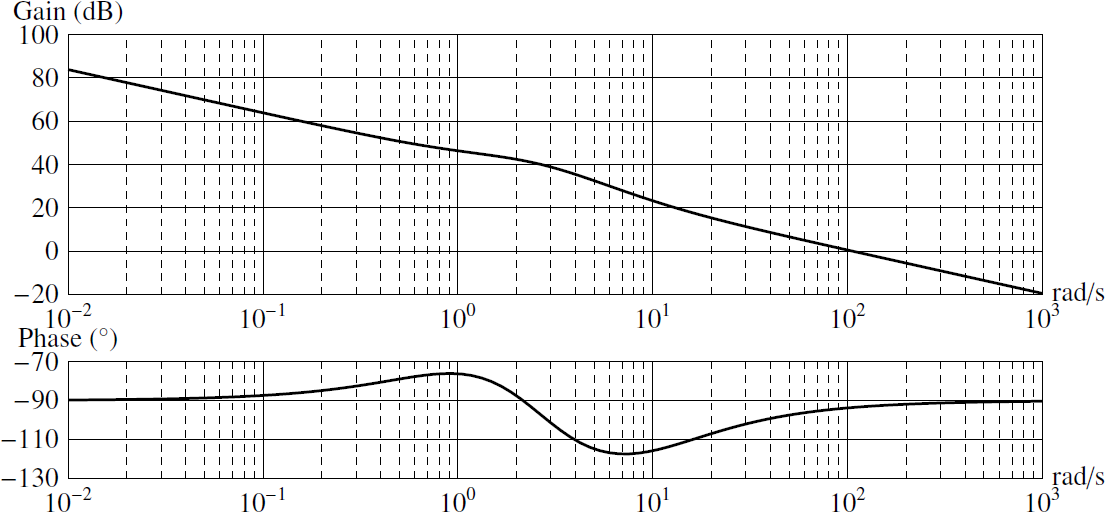
\includegraphics[width=.8\linewidth]{fig_15}
\caption{Diagrammes de Bode en boucle ouverte avec réglage du correcteur PI effectué \label{fig_15}}
\end{figure}


\begin{figure}[H]
\centering
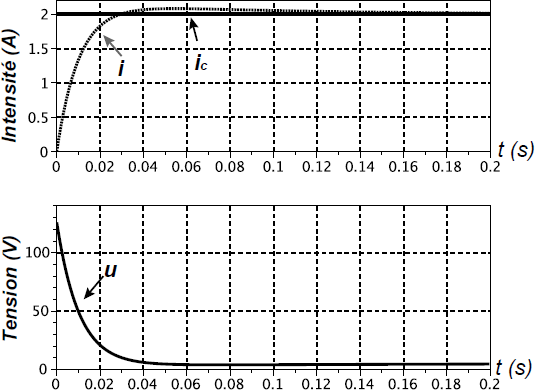
\includegraphics[width=.8\linewidth]{fig_16}
\caption{Réponses temporelles avec réglage du correcteur PI effectué \label{fig_16}}
\end{figure}


\fi

% Q35.
\question{Commenter le résultat obtenu vis-à-vis de l’exigence «~1.7.1.1.4~». Expliquer pourquoi cet asservissement n’est pas directement implanté en l’état dans le système (on pourra s'intéresser à la réponse en tension du du système).}
\ifprof
\begin{corrige}
La marge de phase est respectée. Cependant la tension atteinte demandée par la commande (\SI{120}{V}) est peut être trop élevée pour le moteur. 
\begin{figure}[H]
\centering
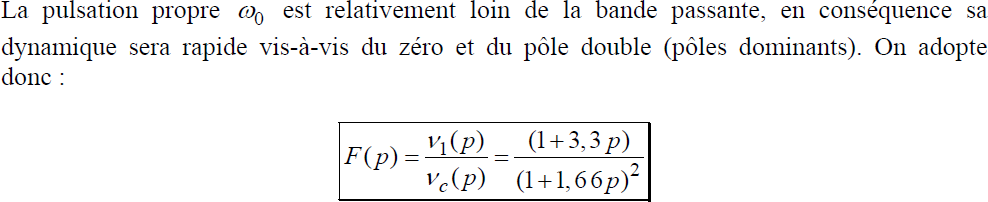
\includegraphics[width=.7\linewidth]{cor_04}
%\caption{Schéma-blocs \label{cor_02}}
\end{figure}
\end{corrige}
\else
\fi


Le correcteur reste inchangé. Afin de palier au problème identifié précédemment, on apporte une dernière évolution au sein du calculateur. Cela permet de respecter les exigences de l’asservissement. \autoref{fig_17} présente les réponses temporelles du système pour un échelon d’intensité $i_c(t)$ de \SI{2}{A}.

%Q36.
\question{Préciser quelle ultime modification a apporté le constructeur afin de respecter les exigences de l’asservissement.}
\ifprof
\begin{corrige}
Le constructeur a ajouté une saturation de $\pm \SI{60}{V}$.
\end{corrige}
\else



\begin{figure}[H]
\centering
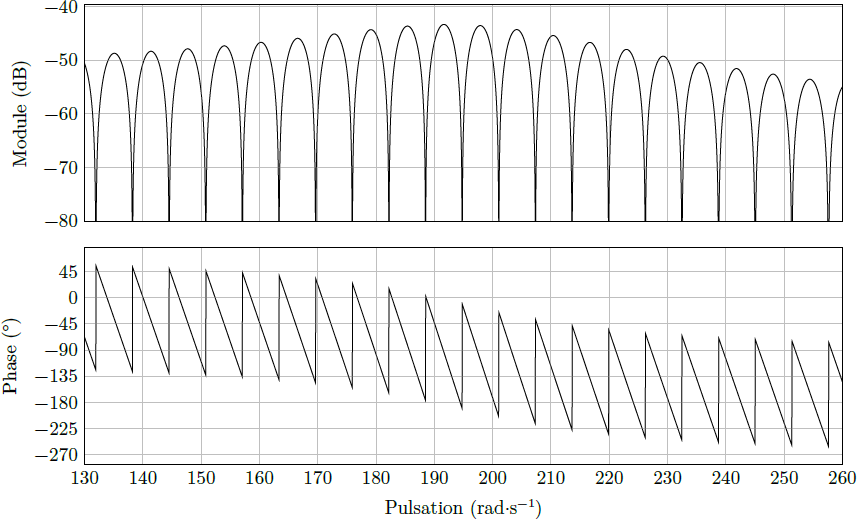
\includegraphics[width=.8\linewidth]{fig_17}
\caption{Réponses temporelles du système finalement implanté\label{fig_17}}
\end{figure}

\fi


\ifprof
\else
\ifcolle
\else
\marginnote{
\begin{solution}
\begin{enumerate}
\item $U(p) = E(p)+RI(p)+Lp I(p)$, $E(p)=K_e\Omega_m(p)$, $C_m(p)=K_e I(p)$, $\indice{J}{eq} p\Omega_m(p) = C_m(p)-f\Omega_m(p)$.
\item .
\item $K_m = \dfrac{f}{Rf+K_e^2}$, $\tau_m=\dfrac{J}{f}$, 
$\omega_{0m} = \sqrt{\dfrac{Rf+K_e^2}{LJ}} $
 $ z_m = \dfrac{Lf + RJ}{2\sqrt{LJ}\sqrt{Rf+K_e^2}}$.
\item $\indice{K}{capt}=\indice{K}{IU}$.
\item $\varepsilon_s = \dfrac{1}{1+K_m K_P \indice{K}{Capt}} $.
\item .
\item .
\item Saturation.
\end{enumerate}
\end{solution}
}
\fi
\fi

\ifprof
\else
\begin{marginfigure}
\centering
\fancyqr{http://xpessoles-cpge.fr/pdf/Cy_01_Ch_02_Colle_04_Hublex_Corrige.pdf}
\end{marginfigure}
\fi
